\documentclass[10pt]{article}
\usepackage[margin=0.72in]{geometry}
\usepackage[T1]{fontenc}
\usepackage{newtxtext,newtxmath}
\usepackage{microtype}
\usepackage{booktabs}
\usepackage{graphicx}
\usepackage{xcolor}
\usepackage{enumitem}
\usepackage[hidelinks]{hyperref}
\definecolor{accent}{HTML}{0F766E}
\setlength{\parindent}{0pt}
\setlength{\parskip}{0.28em}
\setlist[itemize]{leftmargin=1.2em,itemsep=0.12em,topsep=0.12em}
\begin{document}
{\color{accent}\rule{\linewidth}{1.2pt}}

{\Large\bfseries Hybrid Variable Elimination Ordering: v2 Results}

{TTIC 31180 --- Probabilistic Graphical Models Final Project}

{\color{accent}\rule{\linewidth}{0.8pt}}

\section*{What Changed in v2}
Version 2 keeps the v1 baselines and adds three improvements: canonical \texttt{pgmpy} Bayesian-network benchmarks with native cardinalities, a redesigned fill-edge-local pressure term, and diagnostic cheap lookahead / bounded-lookahead runs. The original v1 hybrid penalized all high-degree neighbors; the v2 fill-pressure score penalizes only pressure created by actual fill-in edges, which is intended to reduce brittleness on hub-dominated graphs. The adaptive method chooses $\lambda$ from graph statistics rather than from topology labels.

\section*{Setup}
The v2 run used 71 graph instances and 872 successful method-instance runs. It loaded 5 canonical \texttt{pgmpy} Bayesian networks. Explicit pairwise VE completed for 478 of 872 rows under the factor-size cutoff. The cheap one-step method was run on 15 medium/small rows; bounded-lookahead oracle diagnostics produced 5 rows.

\begin{center}
{\small
\begin{tabular}{lrrrr}
\toprule
\textbf{Benchmark} & \textbf{$n$} & \textbf{Edges} & \textbf{Max card.} & \textbf{Source} \\
\midrule
alarm & 37 & 65 & 4 & pgmpy\_example\_model \\
asia & 8 & 10 & 2 & pgmpy\_example\_model \\
child & 20 & 30 & 6 & pgmpy\_example\_model \\
hailfinder & 56 & 99 & 11 & pgmpy\_example\_model \\
insurance & 27 & 70 & 5 & pgmpy\_example\_model \\
\bottomrule
\end{tabular}
}
\end{center}

\section*{Structural Results}
Lower is better. Tables report topology-level medians.

\begin{center}
{\small
\begin{tabular}{lrrrrrr}
\toprule
\textbf{Topology} & \textbf{Min-degree} & \textbf{Min-fill} & \textbf{Weighted} & \textbf{V1 degree} & \textbf{V2 fill} & \textbf{Adaptive} \\
\midrule
Low-treewidth & 1.0 & 1.0 & 1.0 & 1.0 & 1.0 & 1.0 \\
Random & 22.0 & 20.0 & 21.0 & 21.0 & 21.0 & 21.0 \\
Grid & 11.5 & 11.5 & 11.5 & 11.0 & 12.0 & 11.5 \\
Scale-free & 10.0 & 10.0 & 10.0 & 10.0 & 12.0 & 10.0 \\
Moralized BN & 4.0 & 4.0 & 4.0 & 4.0 & 4.0 & 4.0 \\
\bottomrule
\end{tabular}
}
\end{center}

\begin{center}
{\small
\begin{tabular}{lrrrrrr}
\toprule
\textbf{Topology} & \textbf{Min-degree} & \textbf{Min-fill} & \textbf{Weighted} & \textbf{V1 degree} & \textbf{V2 fill} & \textbf{Adaptive} \\
\midrule
Low-treewidth & 1.40 & 1.40 & 1.40 & 1.40 & 1.40 & 1.40 \\
Random & 10.10 & 10.14 & 10.07 & 10.20 & 8.83 & 10.07 \\
Grid & 5.90 & 5.83 & 5.08 & 4.95 & 4.44 & 5.08 \\
Scale-free & 6.72 & 6.99 & 6.72 & 7.22 & 6.85 & 6.72 \\
Moralized BN & 2.33 & 2.33 & 2.33 & 2.33 & 2.33 & 2.33 \\
\bottomrule
\end{tabular}
}
\end{center}

\section*{Lambda Sensitivity}
The fill-edge-local pressure term shifted the useful $\lambda$ regime. In this run, larger $\lambda$ values helped random and grid graphs more than the original v1 degree-pressure score, while low-treewidth and canonical BN benchmarks still preferred little or no extra pressure.

\begin{center}
{\small
\begin{tabular}{lrr}
\toprule
\textbf{Topology} & \textbf{Best $\lambda$} & \textbf{Median $\log_{10}$ peak size} \\
\midrule
Low-treewidth & 0.00 & 1.40 \\
Random & 1.00 & 8.83 \\
Grid & 1.00 & 4.44 \\
Scale-free & 0.05 & 6.62 \\
Moralized BN & 0.00 & 2.33 \\
\bottomrule
\end{tabular}
}
\end{center}

\section*{Failure Cases}
The table reports $\Delta=\log_{10}(\text{method peak})-\log_{10}(\text{weighted min-fill peak})$ for the worst v1-degree failures. Negative values are improvements over weighted min-fill; positive values are worse.

\begin{center}
{\small
\begin{tabular}{llrrr}
\toprule
\textbf{Topology} & \textbf{Graph} & \textbf{V1 $\Delta$} & \textbf{V2 $\Delta$} & \textbf{Adaptive $\Delta$} \\
\midrule
Random & er\_n120\_p0.10\_s1 & 1.72 & 2.02 & 0.00 \\
Random & er\_n120\_p0.06\_s2 & 1.05 & 0.83 & 0.00 \\
Scale-free & ba\_n150\_m2\_s2 & 0.80 & 0.45 & 0.00 \\
Moralized BN & pgmpy\_insurance & 0.78 & 0.60 & 0.78 \\
Random & er\_n80\_p0.10\_s1 & 0.75 & 0.13 & 0.00 \\
Scale-free & ba\_n100\_m1\_s0 & 0.70 & 0.00 & 0.00 \\
\bottomrule
\end{tabular}
}
\end{center}

\section*{Figures}
\begin{center}
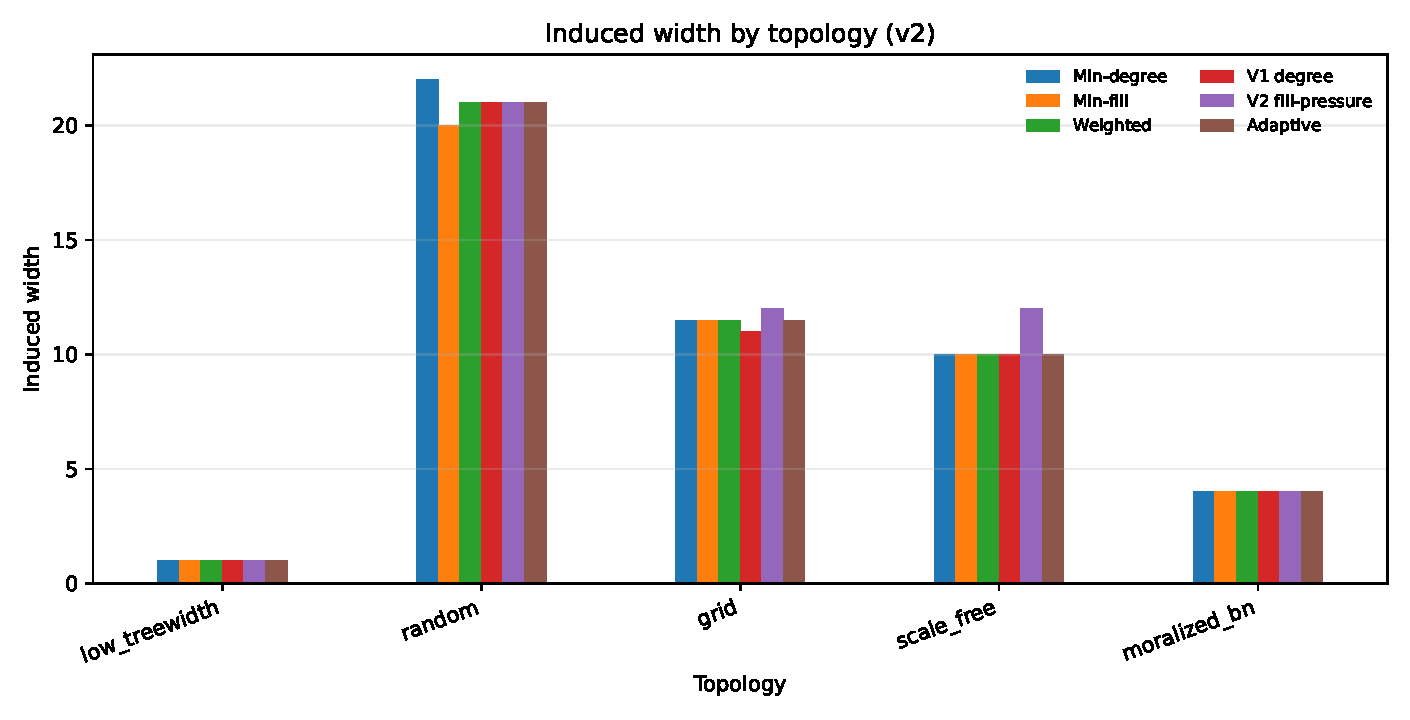
\includegraphics[width=0.92\linewidth]{../figures/v2_induced_width_by_topology.pdf}
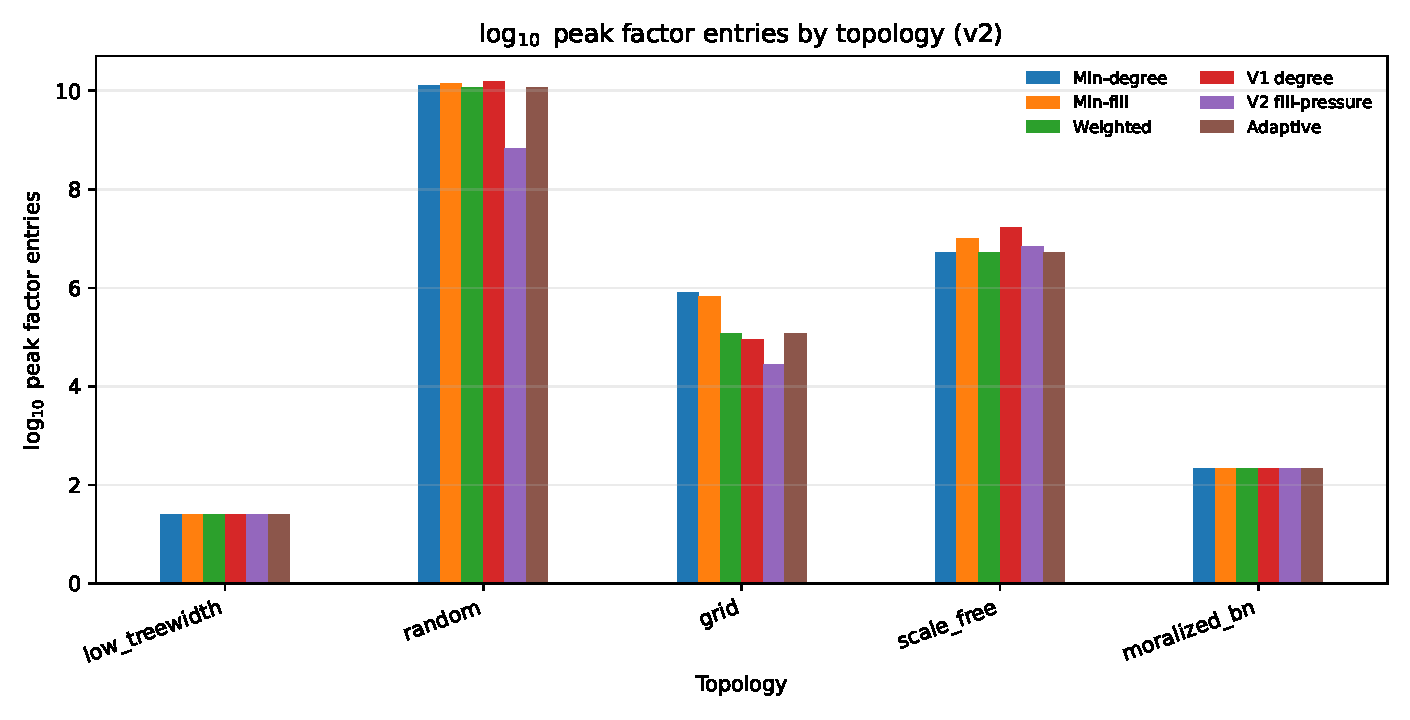
\includegraphics[width=0.92\linewidth]{../figures/v2_peak_factor_by_topology.pdf}
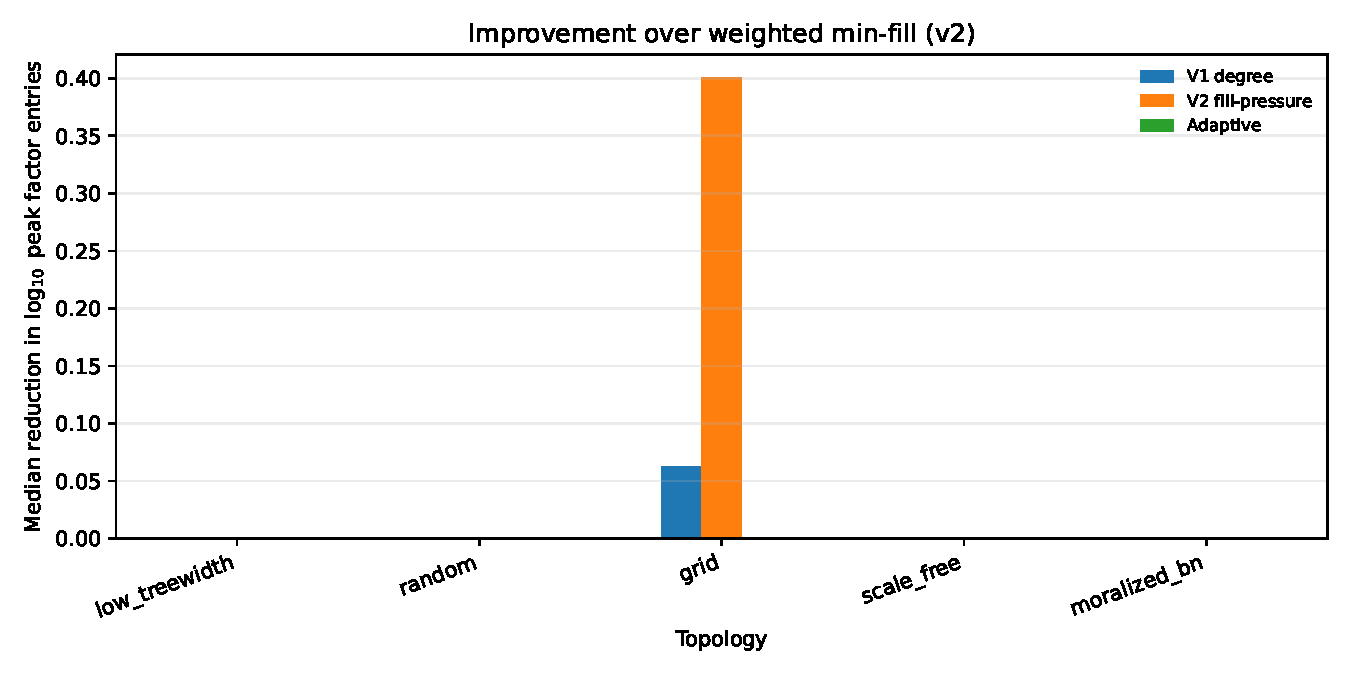
\includegraphics[width=0.92\linewidth]{../figures/v2_improvement_over_wmf.pdf}
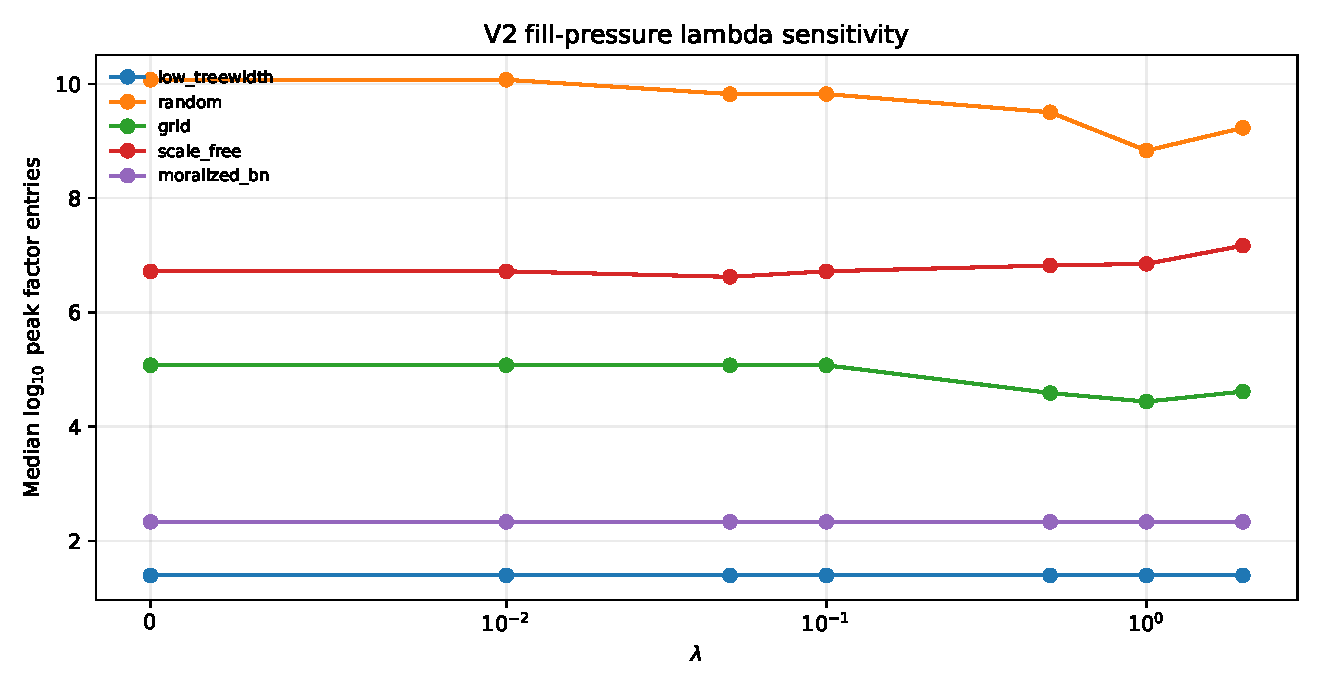
\includegraphics[width=0.92\linewidth]{../figures/v2_lambda_sensitivity.pdf}
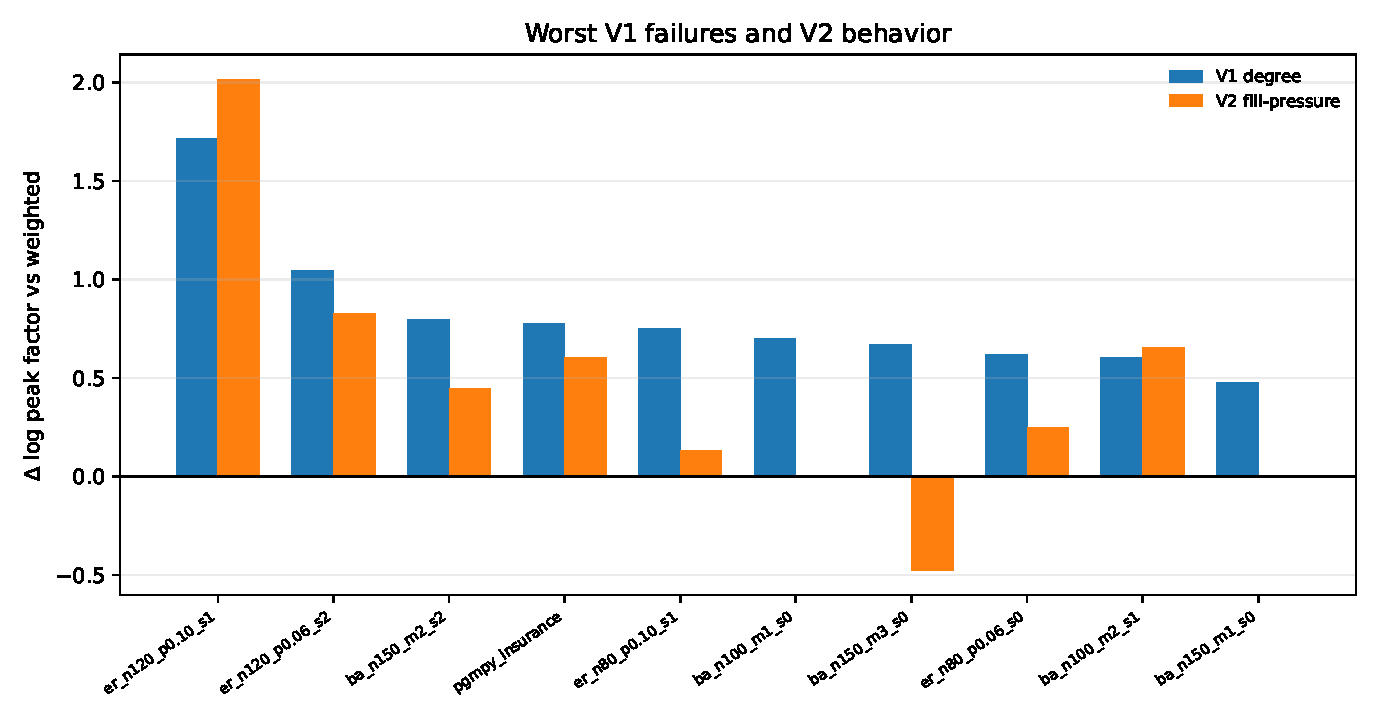
\includegraphics[width=0.92\linewidth]{../figures/v2_failure_cases.pdf}
\end{center}

\section*{Findings and Implications}
\begin{itemize}
\item The topology dependence remains the dominant story. No hybrid method uniformly dominates weighted min-fill.
\item The redesigned fill-pressure term reduces one weakness of v1: it no longer broadly penalizes high-degree neighborhoods when the actual new fill-in is small.
\item A fixed v2 $\lambda=1$ gives stronger median peak-factor results on random and grid graphs than the conservative $\lambda=0.1$ choice from v1, but it is still not a universal setting.
\item Canonical BN benchmarks are less favorable to hybrid pressure: weighted min-fill is already strong, and extra pressure often adds little.
\item Adaptive $\lambda$ is useful as a concept, but the current hand-written rule is not yet reliable enough to replace a sweep. It avoids some v1 hub failures but can still misclassify random or BN-like structure.
\end{itemize}

\section*{Limitations}
The v2 run improves benchmark realism, but it still uses structural pairwise VE instrumentation rather than full CPD-aware BN inference. The next-step heuristic is diagnostic-only on medium/small graphs because full-size one-step simulation was too expensive. The adaptive rule is intentionally simple and should be treated as a prototype rather than a tuned model-selection procedure.

\section*{Next Steps}
\begin{itemize}
\item Replace the hand-written adaptive rule with a small validation-based selector that chooses $\lambda$ from pilot instances by graph statistics.
\item Add CPD-aware exact inference for canonical BNs, or use pgmpy/pyAgrum inference as a runtime validation layer.
\item Expand oracle diagnostics on selected small graphs to compare cheap proxies against explicit lookahead more systematically.
\item Analyze individual elimination traces for the random and insurance failure cases where adaptive fill-pressure is worse than weighted min-fill.
\item Consider a guarded hybrid rule: use weighted min-fill by default, activate pressure only when pilot graph statistics predict a benefit.
\end{itemize}

\end{document}
